\documentclass[12pt]{beamer}

% ****************
% ***** INFO *****
% ****************
\usepackage[english]{babel}
\title[]{Wages, Minimum Wages, and Price Pass-Through:
	The Case of McDonald’s Restaurants}
\subtitle{ECAG-6665: Research Report}
\author[Name Surname]{Alejandro Ouslan}
\institute[institute]{University of Puerto Rico}
\date{} % or \today

% *******************
% ***** PROJECT *****
% *******************
% main color: to black
\definecolor{main}{HTML}{000000}
\setbeamercolor{structure}{fg=main}

% *****************
% ***** THEME *****
% *****************
\usepackage{helvet}
\renewcommand{\familydefault}{\sfdefault}
\setbeamertemplate{frametitle continuation}{\gdef\beamer@frametitle{}}
\setbeamertemplate{footline}{}
\setbeamertemplate{navigation symbols}{}
\usepackage{csquotes}
\usepackage[backend=biber,style=numeric]{biblatex}
\addbibresource{../../reference.bib} % Link to the bibliography file

% *****************
% ***** CODE *****
% *****************
\usepackage{listings}
\lstdefinestyle{py}{
	backgroundcolor=\color{white},
	basicstyle=\ttfamily\scriptsize,
	breaklines=true,
	commentstyle=\color{gray},
	keywordstyle=\color{blue},
	stringstyle=\color{magenta},
	language=Python
}

% **********************
% ***** ALGORITHMS *****
% **********************
\usepackage{algorithm}
\usepackage{algpseudocode}

% *****************
% ***** UTILS *****
% *****************
\usepackage{xcolor}

% ********************
% ***** DOCUMENT *****
% ********************
\begin{document}

% **********************
% ***** TITLEPAGE ******
% **********************
\begin{frame}{}
	\vspace{\fill}

	
\includegraphics[width=0.16\linewidth]{../../assets/uprm_logo.png}

	\vspace{\fill}

	\Large
	\color{main}
	\inserttitle

	\medskip

	\large
	\color{black}
	\insertsubtitle

	\vspace{\fill}

	\footnotesize
	\insertinstitute

	\vspace{\fill}

	\textbf{Author:} \insertauthor

	\medskip

	\insertdate

	\vspace{\fill}
\end{frame}

% *****************
% ***** START *****
% *****************
\begin{frame}[allowframebreaks]{Research Question}
	\begin{itemize}
		\item The research question for this study is whether the minimum wage increase affects the prices of McDonald's products. \cite{ashenfelter2022minimum}
	\end{itemize}

\end{frame}

\begin{frame}[allowframebreaks]{Justification of Research}
	\begin{itemize}
		\item This study provides insight into whether increases of the minimum wage affect the prices of products and determine its elasticity.
		\item The study also provides whether the introduction of labor saving technology like touch screens ordering kiosks affects the price of products.
	\end{itemize}

\end{frame}

\begin{frame}[allowframebreaks]{Literature Review}
	\begin{itemize}
		\item Minimum wage hikes are often associated with a positive spillover (or "ripple effect") on wages above the new minimum \cite{cengiz2019effect}.
		\item Wage spillovers may reflect the value of outside options or within-firm pay norms \cite{flinn2006minimum}
		\item Potential for technological substitution of low-skill labor is limited to cognitively routine tasks, i.e., it may not apply to manually routine jobs. \cite{phelan2019hedonic}
		\item Under monopsonistic competition in local markets, fims face an upward sloping labor supply curve. \cite{manning2013monopsony}
	\end{itemize}

\end{frame}

\begin{frame}[allowframebreaks]{Data Characteristics and Data Sources}
	\begin{itemize}
		\item The data comes form the annual geo-coded listing of all McDonald's restaurants.
		\item The database was obtained from AggData, a market research company
		\item 2016-2020 annual telephone surveys of McDonald's restaurants done by the author of the study.
		\item of these, 720 observations come from stores that are observed only once.
		\item The reliability ration corresponding to annual wage changes is about 0.9.
		\item The survey data was supplemented with data from owner identities by FranData.
	\end{itemize}
\end{frame}

\begin{frame}[allowframebreaks]{Methodology}
	\begin{itemize}
		\item Estimating the McWage elasticity with respect o minimum wages from 2016 to 2020.
		      \begin{equation}
			      \ln{McWage_{it}} = \alpha + \beta \ln{MW_{it}} + \delta_{i} + \phi_{t} + \epsilon_{it}
		      \end{equation}
		\item Estimating a two-stage least square regression of prices on wages where wages are instrumented using minimum wages.
		      \begin{equation}
			      \ln{BigMacPrice_{it}} = \alpha + \beta \ln{McWage_{it}} + \delta_{i} + \phi_{t} + \epsilon_{it}
		      \end{equation}
		\item The reduced form relationship between prices and minimum wages is given by:
		      \begin{equation}
			      \ln{BigMacPrice_{it}} = \alpha + \beta \ln{MW_{it}} + \delta_{i} + \phi_{t} + \epsilon_{it}
		      \end{equation}
		\item Estimate a specification relating the probability of restaurant ecit to minimum wages at the county level.
		      \begin{equation}
			      \ln{Exit_{it}} = \alpha + \beta \ln{MW_{it}} + \delta_{i} + \phi_{t} + \epsilon_{it}
		      \end{equation}
	\end{itemize}

\end{frame}

\begin{frame}[allowframebreaks]{Results Figures}
	\begin{center}
		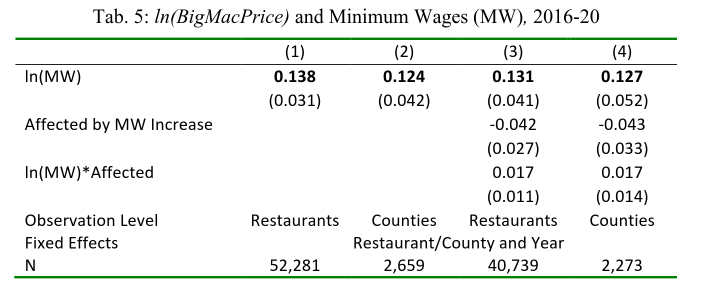
\includegraphics[width=1.0\linewidth]{assets/results.png}
	\end{center}
\end{frame}

\begin{frame}[allowframebreaks]{Descriptive Statistics}
	\begin{center}
		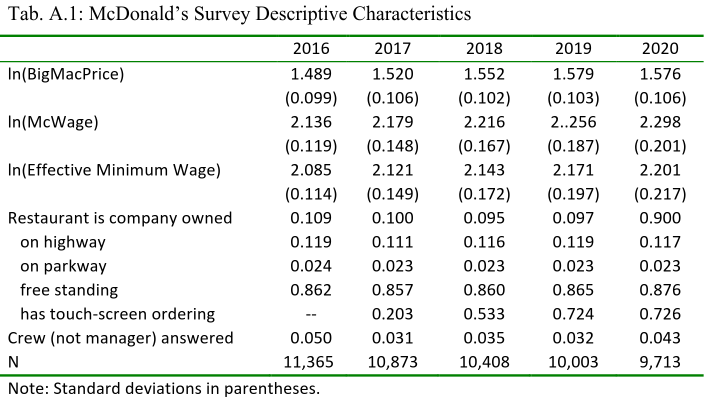
\includegraphics[width=1.0\linewidth]{assets/discriptive.png}
	\end{center}
\end{frame}

\begin{frame}[allowframebreaks]{Results}
	\begin{itemize}
		\item The results show that the McWage elasticity with respect to minimum wages is 0.3.
		\item The results also show that the price elasticity of Big Mac prices with respect to McWages is 0.1.
		\item The results also show that the price elasticity of Big Mac prices with respect to minimum wages is 0.03.
	\end{itemize}
\end{frame}

\begin{frame}[allowframebreaks]{Graphs}
	\begin{center}
		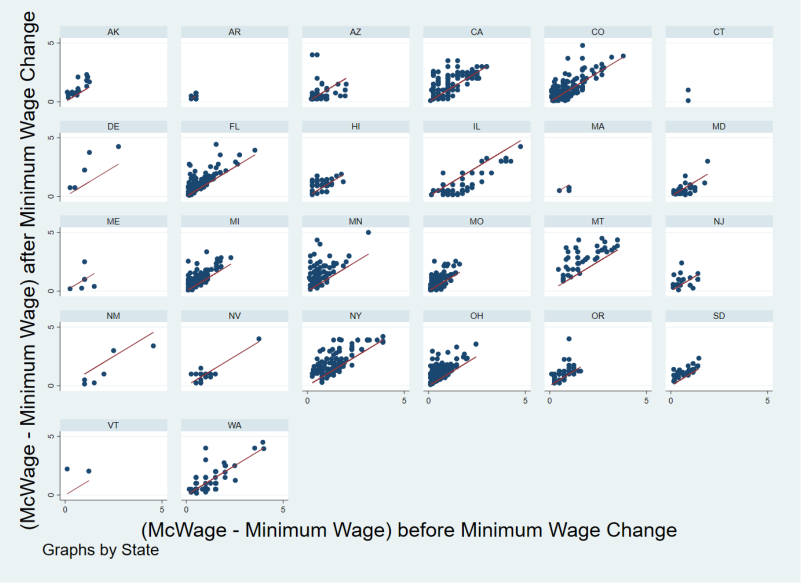
\includegraphics[width=1.0\linewidth]{assets/graphs.png}
	\end{center}
\end{frame}

\begin{frame}[allowframebreaks]{Conclusions}
	\begin{itemize}
		\item  McDonald's restaurants adjust wages in response to minimum wage hikes, with a 0.68 elasticity of McWages. Many maintain a wage "premium" above the minimum wage, reflecting spillover effects on pay norms across employers and employee turnover.
		\item Despite higher labor costs from minimum wage increases, McDonald's restaurants do not adopt labor-saving technology like touch-screen ordering, and there is no evidence of restaurant closures. The elasticity of Big Mac prices with respect to labor cost increases is high, indicating strong price pass-through.
	\end{itemize}
\end{frame}
% ************************
% ***** BIBLIOGRAPHY *****
% ************************
\begin{frame}[allowframebreaks]{Bibliography}
	\printbibliography
\end{frame}
% ***************
% ***** END *****
% ***************

\end{document}
